\documentclass[a4paper,12pt]{article}

% General document formatting
%\usepackage[margin=0.7in]{geometry}
\usepackage[parfill]{parskip}
\usepackage{url, hyperref}
\usepackage{color}
\usepackage[usestackEOL]{stackengine}[2013-10-15] % formatting Pascal
\usepackage[dvipsnames]{xcolor}

\usepackage{cancel}
\usepackage[export]{adjustbox}

\usepackage{csquotes}

% Related to math
\usepackage{amsmath,amssymb,amsfonts,amsthm}
\usepackage{mathtools}
\usepackage{tikz}
\usetikzlibrary{arrows,matrix,positioning}
\DeclarePairedDelimiter\norm{\lVert}{\rVert}
\newcommand{\innerproduct}[2]{\langle #1, #2 \rangle}
\usepackage{algorithm}
\usepackage{algorithmicx}
\usepackage{algpseudocode}
\usepackage{listings}
\usepackage{breqn} % for equation breaking
\usepackage[linguistics]{forest} %trees

\lstdefinestyle{matlab}{
  language=Matlab,
  basicstyle=\ttfamily,
  keywordstyle=\color{blue},
  commentstyle=\color{green!50!black},
  stringstyle=\color{red},
  showstringspaces=false,
  numbers=left,
  numberstyle=\tiny\color{gray},
  stepnumber=1,
  numbersep=5pt,
  breaklines=true,
  breakatwhitespace=true,
  tabsize=2,
  frame=single,
  captionpos=b,
  columns=fullflexible
}



\algdef{SE}[DOWHILE]{Do}{doWhile}{\algorithmicdo}[1]{\algorithmicwhile\ #1}%

% encoding and language
\usepackage{lmodern}
\usepackage[slovene]{babel}
\usepackage[utf8]{inputenc}
\usepackage[T1]{fontenc}
\usepackage[mathscr]{euscript}

% multiline comments
\usepackage{verbatim}

% images
\usepackage{graphicx}
\graphicspath{ {./images/} }

% tags
\usepackage{pifont}
% \tag{\ding{37}} - telefon

% theorems
\theoremstyle{definition}
\newtheorem{counter}{Counter}[section] % not for use
\newtheorem{definition}[counter]{Definition}
\newtheorem{lemma}[counter]{Lemma}
\newtheorem{conseq}[counter]{Consequence}
\newtheorem{claim}[counter]{Claim}
\newtheorem{theorem}[counter]{Theorem}
\newtheorem{example}[counter]{Example}
\newtheorem{corollary}[counter]{Corollary}
\newtheorem{proposition}[counter]{Proposition}
%%
\theoremstyle{remark}
\newtheorem*{ex}{Example}
\newtheorem*{remark}{Remark}
%\newtheorem*{problem}{Problem}
\newtheorem{rem*}[counter]{Remark}
%\newtheorem{ex*}[counter]{Primer}

% I like my squares DARK
\renewcommand\qedsymbol{$\blacksquare$}

% common commands redefined convenience purposes
\newcommand{\N}{\mathbb{N}}
\newcommand{\Z}{\mathbb{Z}}
\newcommand{\Q}{\mathbb{Q}}
\newcommand{\R}{\mathbb{R}}
\newcommand{\C}{\mathbb{C}}
\newcommand{\Pp}{\mathbb{P}}
\newcommand{\ch}{\operatorname{char}}

% subsubsubsections (paragraphs)
\usepackage{titlesec}
\usepackage{hyperref}

\titleclass{\subsubsubsection}{straight}[\subsection]

\newcounter{subsubsubsection}[subsubsection]
\renewcommand\thesubsubsubsection{\thesubsubsection.\arabic{subsubsubsection}}
\renewcommand\theparagraph{\thesubsubsubsection.\arabic{paragraph}} % optional; useful if paragraphs are to be numbered

\titleformat{\subsubsubsection}
  {\normalfont\normalsize\bfseries}{\thesubsubsubsection}{1em}{}
\titlespacing*{\subsubsubsection}
{0pt}{3.25ex plus 1ex minus .2ex}{1.5ex plus .2ex}

\makeatletter
\renewcommand\paragraph{\@startsection{paragraph}{5}{\z@}%
  {3.25ex \@plus1ex \@minus.2ex}%
  {-1em}%
  {\normalfont\normalsize\bfseries}}
\renewcommand\subparagraph{\@startsection{subparagraph}{6}{\parindent}%
  {3.25ex \@plus1ex \@minus .2ex}%
  {-1em}%
  {\normalfont\normalsize\bfseries}}
\def\toclevel@subsubsubsection{4}
\def\toclevel@paragraph{5}
\def\toclevel@paragraph{6}
\def\l@subsubsubsection{\@dottedtocline{4}{7em}{4em}}
\def\l@paragraph{\@dottedtocline{5}{10em}{5em}}
\def\l@subparagraph{\@dottedtocline{6}{14em}{6em}}
\makeatother

\setcounter{secnumdepth}{4}
\setcounter{tocdepth}{4}

% f|_{nekaj}
\newcommand\restr[2]{{% we make the whole thing an ordinary symbol
  \left.\kern-\nulldelimiterspace % automatically resize the bar with \right
  #1 % the function
  \littletaller % pretend it's a little taller at normal size
  \right|_{#2} % this is the delimiter
  }}

  \newcommand{\littletaller}{\mathchoice{\vphantom{\big|}}{}{}{}}

\begin{document}

\begin{titlepage}
    \begin{center}
        
        \vspace*{3cm}
            
        \Huge
        \textbf{Računska zahtevnost}

        \large
        Zapiski s predavanj prof. Alexandra Simpsona

        \vspace*{0.5cm}
        \LARGE
        Domen Vogrin

        \vfill
        \normalsize
        Ljubljana, jesen 2023
    \end{center}

\end{titlepage}

\clearpage

\pagenumbering{roman}
\tableofcontents
\newpage
\pagenumbering{arabic}


% 2. 10. 2023
\section{Basics}
\subsection{Determinant of a matrix}
Determinant of matrix
\begin{equation*}
    A = \begin{bmatrix}
        a_{11} & \cdots & a_{1n} \\
        \vdots & \ddots & \vdots \\
        a_{n1} & \cdots & a_{nn}
    \end{bmatrix}
\end{equation*}

is calculated via formula

\begin{equation*}
    det(A) = \sum_{\sigma \in perm(n)} sgn(\sigma) \cdot \prod_{i = 1}^{n} a_{i, \sigma(i)}
\end{equation*}

Naive algorithm requires $n! \cdot (n-1)$ multiplications, which is worse than exponantional. However, there are better algorithms for the permanent.
Use Gaussian elimination to factorise $A$

\begin{equation*}
    A = L \cdot U \cdot P
\end{equation*}

where $L$ is lower triangle matrix, $U$ is upper triangle matrix, and $P$ is a permutation. This helps, because
\begin{align*}
    det(A) =& det(L) \cdot det(U) \cdot det(P) \\
           =& det(L) \cdot det(U)
\end{align*}
We can compute determinants of $L$ and $U$ by just multiplying diagonal elements.

Time complexity od $LU$ decomposition is $\mathscr{O}(n^3)$, which is also time complexity of our algorithm.

Fastest known time for determinant is $\mathscr{O}(n^{2,376})$.

\subsection{Primality testing}
For given $n$, is $n$ prime?

Naive algorithm: Count through the odd nimbers from 3 up to $\sqrt{n}$ and check that none divides $n$. This gives us naive time complexity of $\mathscr{O}(\sqrt{n})$.
But the appropriate size measure is $|n|$, which is the length of $n$. This means, that naive algorithm is exponential in $|n|$.

There are clever more efficient algorithms:
\begin{itemize}
    \item The algorithm used in practice (Miller-Rabin) uses randomness, and has a positive probability of error. (1970s)
    \item Breakthrough in 2002 the AKS algorithm: a deterministic polynomial-time algorithm for primality testing.
\end{itemize}

\subsection{Prime factorisation}
For given $n$, compute the list (with multiples) of its prime numbers.

For given $n$, return two numbers smaller than $n$ whose product is $n$ (if such exist), 0 otherwise. It is an open problem if exist an efficient
deterministic/algorithm algorithm to solve this problem.

However, Shor's algorithm (1994) is an efficient quantum algorithm.

\subsection{K-colourability}

E.g. 3-colourability.

It is an open question if there exists an efficient deterministic (random) algorithm for 3-colourability (or for k-colourabilits if $k \geq 3$).

Equivalent statement: P = NP

These statements are equivalent, because 3-colourability is NP-complete.

Related questions:
\begin{itemize}
    \item Decision problem: Is a given graph 3-colourable (Does there exists a solution)
    \item Search problem: Given a graph, find a 3-colouring (if one exists, otherwise return ``I can't'')
    \item Counting problem: Count the number of 3-colourings
    \item Sampling problem: Find a random (w.s.t. uniform distribution) 3-colouring.
\end{itemize}

\subsection{Perfect matchings}
Given a bipartite graph (two sided)

A perfect matching is a bijection netween the two sides that follows the edges of the graph.

\begin{itemize}
  \item Decision problem: efficient algorithm exsists, because
  \item Search problem: efficion algorithm exsists (Ford-Falkerson for network flow ...)
  \item Counting problem: Open question ($FP \neq \#P$)
\end{itemize}

We can represent the bipartite graph as an adjacency matrix.

Number of perfect matchings is 
\begin{equation*}
  \sum_{\sigma = perm(n)} \prod_{i = 1}^{n} a_{i, \sigma(i)} = perm(A)
\end{equation*}
which is a permanent of $A$.


\section{Asymptotic notation}
measures rate of growth.

Typically we want to relate a function
\begin{equation*}
    T: \N \to \R
\end{equation*}

to a more mathematically natural
\begin{equation*}
    f: \N \to \R
\end{equation*}

\subsection{Big o notation}
Main definition:
\begin{equation*}
    T(n) = \mathscr{O}(f(n)) \iff \exists N \: \exists c > 0 \text{ s.t. } \forall n \geq N \; T(n) \leq c \cdot f(n)
\end{equation*}

This is big $\mathscr{O}$ notation.

We are really saying $T \in \mathscr{O}(f)$.

%Polynomial growth (daj O(n) \pod O(n^2) ...)
%quasi polynomial
%Exponential growth
% doubly exponential

\subsection{Little o notation}
Main definition:
\begin{equation*}
    T(n) = o(f(n)) \iff \forall c > 0 \: \exists N \text{ s.t. } \forall n \geq N \; T(n) \leq c \cdot f(n)
\end{equation*}

We are really saying $T \in o(f)$.






\newpage

% 9.10.2023 

\subsection*{How hard is it to solve computational problems?}

We are interested in the resources used, in particular time and space. We need a mathematical model of what an algorithm is that supports an analysis
of time and space.

\section{Turing machines (1936)}

Turing machine is algorithm by definition, sort of computer that runs a fixed program.

\begin{itemize}
    \item An algorithm should be a finite description of a computational process.
    \item The algorithm should specify the computational process in its entirety.
    \item The process of following algorithm should be carried out without any creative input.
    \item So it is a process that can be carried out by a suitable machine.
    \item Machine will perform steps in time and need enough working space to carry out calculations.
    \item We do not bound time and space in advance.
\end{itemize}

\begin{definition}
    A (deterministic) Turing machine (TM) is specified by:
    \begin{itemize}
        \item A finite tape alphabet $\Gamma$ with $\square \in \Gamma$ ($\square$ is a blank symbol)
        \item A finite set $Q$ of states with start $\in Q$.
        \item A partial function $\delta: Q \times \Gamma \to Q \times \Gamma \times \{-1, 0, +1\}$.
    \end{itemize}
\end{definition}

A machine configuration is a triple $(q, t, i)$ where
\begin{itemize}
    \item $q \in Q$
    \item $t$ is a tape configuration
    \item $i$ is the position of the head.
\end{itemize}

A tape configuration is a $t: \Z \to \Gamma$ so that $t(m) \neq \square$ for only finitely many $m$.

\subsection{Turing machine execution}
We start the machine in a machine configuration $(q, t, i)$, where $q = start$ and $i$ points at the left-most non $\square$ symbol
on the tape
\begin{equation*}
    i = min\{m \in \Z: t(m) \neq \square\}
\end{equation*}
(if the tape is empty, $i$ can be arbitrary.)

One can define mathematically what it means that $\delta$ takes us from machine configuration $(q, t, i)$ to $(q', t', i')$ and
what it means that $\delta$ halts machine configuration $(q, t, i)$.

\subsection{Using a TM as a language recogniser}
We assume an input alphabet $\Sigma \subseteq \Gamma \setminus \{\square\}$.

(A language is a subset $L \subseteq \Sigma^*$)

We also assume distinguisged halting states accept, reject $\in Q$.

A TM M decides the language $L$ if for any input word $w \in \Sigma^*$
\begin{itemize}
    \item if $w \in L$ then M halts in the accept state on input $w$.
    \item if $w \notin L$ then M halts in the reject state on input $w$.
\end{itemize}

A language is decideable, if there exist a TM M that decides it.

\subsection{Using TMs to compute functions}
Assume an input alphabet $\Sigma_1$ and optput alphabet $\Sigma_2$ with $\Sigma_1, \Sigma_2 \subseteq \Gamma \setminus \{\square\}$.
A TM M computes a function $f: \Sigma_1^* \to \Sigma_2^*$ if
\begin{itemize}
    \item for any $q \in \Sigma_1^*$, when given $w$ as input M eventually halts with $f(w)$ on the tape.
    \item $f$ is computable if there exists a TM that computes $f$.
\end{itemize}

\subsection{Variant Turing Machines}
\begin{itemize}
    \item Machines in which the tape is infinite in only one direction
    \item Machines with $K$ tapes (one head per tape)
    \item Machines with $K$ tapes and many heads per tape, allowing heads to move between tapes
    \item Machines with multidimensional workspaces instead of one dimentional tapes
    \item etcetera $\dots$
\end{itemize}
All such variants are equivalent.

In general a K-tape machine has $K$ tapes each with its own head. So a machine configuration is of the form 
$(q, t_1, \dots, t_k, i_1, \dots, i_k)$ ($k$ tape configurations and $k$ head positions).
Transition function has form
\begin{equation*}
    \delta: Q \times \Gamma^k \to Q \times \Gamma^k \times \{-1, 0, +1\}^k
\end{equation*}
We execute the machine in the ``natural way'' as in the example (not written).

\begin{definition}
    If M is a (k-tape) language recognising TM we define $time_M: \N \to \N$:
    \begin{equation*}
        time_M(n) = max \{\text{no. of steps taken by input }w: w \in \Sigma^*,  |w| = n\}
    \end{equation*}

    For a language $L \subseteq \Sigma^*$ and a function $T: \N \to \N$ we say that $L \in DTime(T(n))$ if there exist $k-tape$ TM M for
    some $k \geq 1$ that decides $L$ such that $time_M(n) = \mathscr{O}(T(n))$.
\end{definition}

\begin{definition}[Fundemental def.]
    \begin{equation*}
        P := \bigcup\limits_{d \geq 1} DTime(n^d)
    \end{equation*}
\end{definition}

Equivalent between machine models proved by translations between models. Such translations do not preserve $DTime(T(n))$. But 
all translations are polynomially bounded in space and time. So the class $P$ is invarient under choice of computational model.






\newpage
% 16.10.2023
\section{Nondeterminism}
An nondeterministic TM (NTM) is:
\begin{itemize}
    \item $\Gamma$ as before
    \item $Q$ as before
    \item $A$ subset $\Delta \subseteq (Q \times \Gamma) \times (Q \times \Gamma \times \{-1, 0, +1\})$
\end{itemize}

The transition relation: for every $(q, a) \in Q \times \Gamma$ there is a finite set of $(q', a', d')$, so that
$((q, a), (q', a', d')) \in \Delta$. Notation: $(q, a) \to (q', a', d')$

Machine configurations are as before.

A run of the machine is a sequence of configurations starting in the starting configuration and respecting the 'rules' of the 
transition relation, whose last configuration, if it exists, is a halting/terminating configuration.

NTMs potentially have many different runs from the same starting configuration.


\subsection{NTMs as language recognisers}

Assume input alphabet $\Sigma \subseteq \Gamma \setminus \{\square\}$ and halting states $accept, reject \in \Q$

An NTM M accepts a word $w \in \Sigma^*$ if there exists a run of M on input $w$ that terminates in accept.

An NTM M rejects a word $w \in \Sigma^*$ if every run of input $w$ terminates in reject.

An NTM M decides the language $L \subseteq \Sigma^*$ if for every $q \in \Sigma^*$:
\begin{itemize}
    \item if $w \in L$ then M accepts w
    \item if $w \notin L$ then M rejects w
\end{itemize}


If M is a NTM, define $\text{time}_M: \N \to \N \cup \{\infty\}$
\begin{dmath*}
    \text{time}_M(n) = max \{\text{no. of steps in the run } r | w \in \Sigma^*, |w| = n, r \text{ is a run of M on input } w\}
\end{dmath*}

For a language $L \subseteq \Sigma^*$ and function $T(N): \N \to \N$, we say that $L \in \text{NTime}(T(n))$ if there exists a NTM M
that decides L such that $\text{time}_M(n) = \mathscr{O}(T(n))$.

\begin{equation*}
    NP := \bigcup\limits_{k} NTime(n^k)
\end{equation*}

\begin{equation*}
    P \subseteq NP
\end{equation*}

because every deterministic TM is nondeterministic.

Big question is:
\begin{equation*}
    P = NP
\end{equation*}

\begin{example}
    Independent set problem - INDSET.

    Input: A graph $G$ and a natural number $k \leq |G|$ - number of vertices of G.

    Question: Does $G$ have an independent set of size $k$.

    An independant set or anticlique is a subset $I$ of the vertices of $G$ such that no two elements of $I$ have an edge between them.

    We code this up as a decision problem for a language over $\{0, 1, \texttt{,}, \texttt{;}\}$

    Example encoding (not here) ->
    Represent a graph as an adjecent matrix.
    Our input word is 010,101,010;10 (before; is matrix, after; is number of vertices)

    If G has $n$ vertices, then our input size is $m^2 + m + \lfloor log_2 k \rfloor + 1$.

    We write $\ulcorner$(G, k)$\urcorner$ for the encoding in $\Sigma^*$ representing the input G, k

    % Poskusi najti boljsi nacin
    INDSET:
    \begin{dmath*}
        \{w \in \{0, 1, ,, ;\}* | w \text{ is of the form } \ulcorner (G, k) \urcorner \text{ where G is a graph with an independent set of size k}\}
    \end{dmath*}

    We now argue that INDSET belongs to NP.

    Given an input word
    \begin{equation*}
        a_1 \dots a_M, \dots
    \end{equation*}

    Scan to the first comma and count number of characters to obtain M as we go along write a nondeterministic sequence of binary bits on second tape. $\mathscr{O}(m)$

    Test to see that there are exactly $k$ 1s on the second tape (if not -> reject). $\mathscr{O}(m^2)$

    For each pair of 1s on the second tape, check that there is a $0$ in the relevant entry in the adjacency matrix on the first tape. $\mathscr{O}(m^4)$

    If so, we accept (otherwise reject)

    The time bound is $\mathscr{O}(m^4)$, ie $\mathscr{O}(n^2)$ (because of input is $m^2$)
\end{example}

\begin{theorem}[Certificate chatacterisation of NP]
    T.f.a.e. for $L \subseteq \Sigma^*$
    \begin{enumerate}
        \item $L \in NP$
        \item There is a polynomial $p(n): \N \to \N$ and a polynomial time bounded deterministic TM such that for any input $w \in \Sigma^*$ t.f.a.e.
        \begin{itemize}
            \item[(a)] $w \in L$
            \item[(b)] there exists certificate $v \in \Sigma^{p(|w|)}$ such that M accepts w, v
        \end{itemize}
    \end{enumerate}

\end{theorem}

\begin{proof}
    (2) -> (1) Nondeterministically generate $v \in \Sigma^{p(|w|)}$. Then deterministically check if it is a solution.
    (1) -> (2) Use the sequence of nondeterministic choices as the certificate.
\end{proof}






\newpage
% 23.10.2023 %
P problems solvable in deterministic polynomial time, NP problems solvable in nondetrministic polynomial time.

\begin{equation*}
    L \in P \iff L \in DTime(p(n))
\end{equation*}

Problems we can efficiently solve.

\begin{equation*}
    L \in NP \iff L \in NTime(p(n))
\end{equation*}


Problems for which we can efficiently verify the correctness of a solution.

This intuition is embodied in the certificate characterisation of LP.

\section{Meet some NP problems}
All these problems are in fact NP-complete.

Main theorem today: Levin theorem: SAT is NP-complete.

Important today: the notions of NP hardness, polynomial time reducibility.

\subsection{SAT}

A propositional formula is
\begin{itemize}
    \item a boolean variable: $u, u', u'', u''', u'''', ...$
    \item a truth value: $1$ (true), $0$ (false)
    \item if $\phi, \psi$ formulas then so are $\phi \cup \psi, \phi \cap \psi, \neg \phi$
\end{itemize}

If we assign truth values $\{0, 1\}$ to propositional variables
\begin{equation*}
    v: \text{variables} \to \{0, 1\}
\end{equation*}
then we compute $v(\phi)$ using truth tables.

$\phi$ is satisfiable, if there exists an assignment $v:$ variable $\to \{0, 1\}$, such that $v(\phi) = \neg$.
We call $v$ a satisfying assignment for $\phi$.

\begin{example}
    $(u \land u') \lor (u \land u'') \lor (u' \land u'')$
    This is satisfiable. $v$ is a satisfying assignment $\equiv$ if maps at least two variables to 1.
\end{example}

\begin{example}
    $u \land \neg u$
    This is not satisfiable.
\end{example}

The SAT problem:
\begin{itemize}
    \item Input: a propositional formula $\phi$
    \item Question: is $\phi$ satisfiable?
\end{itemize}

We represent SAT as a language over the aplhabet $\sigma_{SAT} = \{0, 1, \land, \lor, \neg, u, '\}$

\begin{equation*}
    u \land (u'' \lor u''') \phi
\end{equation*}

represent as the

\begin{equation*}
    \land u \lor u'' u''' \phi'
\end{equation*}

\begin{equation*}
    SAT = \{\phi' | \phi \text{ is a satisfiable formula}\}
\end{equation*}

\subsection*{SAT $\in$ NP}

A certificate for the satisfiability of a formula $\phi$ containing variables up to $u_k$ is simply a word $v \in \{0, 1\}^*$
representing a stisfying assignment.

We can verify in deterministic polynomial time given input $\phi'$, $v$ wheter or not $v$ is a satisfying assignment for $\phi$.

SAT $\in$ NP by the certificate definition of NP.

\subsubsection*{Polytime reducibility}
We say that a language $L_1 \subseteq \Sigma_1^*$ is polynomial-time (ptime) reducible to a language $L_2 \subseteq \Sigma_2^*$ if there exists
a deterministic TM M that compute a function $f: \Sigma_1^* \to \Sigma_2^*$, such that
\begin{itemize}
    \item for all $w \in \Sigma_1^*$:
    \begin{equation*}
        f(w) \in L_2 \iff w \in L_1
    \end{equation*} and
    \item M is polynomial time bounded
    \begin{equation*}
        \exists K \text{ s.t. } time_M(n) = \mathscr{O}(n^K)
    \end{equation*}
\end{itemize}

\subsubsection*{Observations}
\begin{itemize}
    \item $L \leq_p L$
    \item If $L_1 \leq_p L2$ and $L_2 \leq_p L_3$, then $L_1 \leq_p L_3$
    \item If $L' \leq_p L \in P$ then $L' \in P$
    \item If $L' \leq_p L \in NP$ then $L' \in NP$
    \item If $L$ is NP hard and $L \leq_p L'$, then $L'$ is also NP hard
\end{itemize}

\subsubsection*{NP hardness}

$L$ is NP hard, if for any NP language L' we have $L' \leq_p L$.

\subsubsection*{NP completness}

$L$ is NP complete, if $L \in NP$ and L is NP hard.

\begin{theorem}[Cook/Levin]
    SAT is NP complete.
\end{theorem}

\subsection{3-SAT}

A \underline{literal} is a propositional vaiable $u_i$ or its negation $\neg u_i$.

A \underline{clause} is a disjunction $l_1 \lor \dots \lor l_k$ of literals.

A formula is in \underline{conjunctive normal form} (CNF) if it is a conjunction $D_1 \land \dots \land D_m$ where each $D_i$ is a clause.

A 3-clause is a disjunction $l_1 \lor l_2 \lor l_3$ of exactly 3 (not necessarily distinct) literals.

A formula is in \underline{3-CNF} if it is a conjunction $D_1 \land \dots \land D_m$ of 3-clauses.

\textbf{3-SAT}:
\begin{itemize}
    \item Input: a propositional formula in 3-CNF
    \item Question: is the formula satisfiable?
\end{itemize}

\textbf{SAT $\leq_p$ 3-SAT} - The Tseytin transformation.

\begin{example}
    Input: $\lnot (u \lor \lnot u') \lor (u \land \lnot u')$

    From this, we build a tree:
    \begin{forest}
        [$x_0$: $\lor$
            [$x_1$: $\lnot$
                [$x_2$: $\lor$
                    [$u$]
                    [$x_3$: $\lnot$
                        [$u'$]
                    ]
                ]
            ]
            [$x_4$: $\land$
                [$u$]
                [$x_5$: $\lnot$
                    [$u'$]
                ]
            ]
        ]
    \end{forest}

    Idea behind this tree:
    \begin{align*}
        &x_0 \\
        &\land (x_0 \leftrightarrow x_1 \lor x_2) \\
        &\land (x_1 \leftrightarrow \lnot x_2) \\
        &\land (x_2 \leftrightarrow u \lor x_3) \\
        &\land (x_3 \leftrightarrow \lnot u') \\
        &\land (x_4 \leftrightarrow u \land x_5) \\
        &\land (x_5 \leftrightarrow \lnot u')
    \end{align*}

    Output:

    $(x_0 \lor x_0 \lor x_0) \land
    (\lnot x_0 \lor x_1 \lor x_4) \land
    (\lnot x_1 \lor x_0 \lor x_0) \land
    (\lnot x_4 \lor x_0 \lor x_0) \land \\
    (\lnot x_1 \lor x_2 \lor x_2) \land
    (x_2 \lor x_1 \lor x_1) \land
    (\lnot x_2 \lor u \lor x_3) \land
    (\lnot u \lor x_2 \lor x_2) \land \\
    (\lnot x_3 \lor x_2 \lor x_2) \land
    (\lnot x_3 \lor \lnot u' \lor \lnot u') \land
    (u' \lor x_3 \lor x_3) \land
    (\lnot x_4 \lor u \lor u) \land \\
    (\lnot x_4 \lor x_5 \lor x_5) \land
    (\lnot u \lor \lnot x_5 \lor x_4) \land
    (\lnot x_5 \lor \lnot u' \lor \lnot u') \land
    (u' \lor x_5 \lor x_5)$
\end{example}

\subsection{3-COL}

Given a cojnunction of 3-clauses $\phi$. Convert it to a graph that is 3-colourable iff $\phi$ is satisfiable.

Suppose $\phi$ has variables up to $u_k$.

\begin{proof}(that SAT is NP hard)

    Suppose $L \in NP$. We show $L \leq_p SAT$.

    Let M be a single-tape ND TM that decides L with time bound $p(n) \geq time_M(n)$. (p a polynomial).

    If we run M on input $w$.

    The machine can only during its execution look at squares between $-p(n)$ and $p(n)$.

    Modify M so that from any halting state it makes a dummy step (does nothing). We will call it M'.

    Given an input word $w \in \Sigma$ we construct a propositional formula $\Phi_w$ such that
    \begin{align*}
        \Phi_w  \text{ satisfiable} \iff& \text{there exists a run of M' on input w} \\
                                       &\text{that is in the accept state after } p(|w|) \text{ step } \\
                                   \iff& w \in L
    \end{align*}

    $\Phi_w$ will use $(p(|w|) + 1) \times |Q| + (p(|w|) + 1) \cdot (2p(|w|) +1) \cdot (|\Gamma| + 1)$ variables. This
    is polynomial in $|w|$ $\mathscr{O}((p(n))^2)$.

    Mnemonic names for the variables:
    \begin{itemize}
        \item ($\text{state}_t = q$) for every $t = 0 \dots p(|w|)$, $q \in Q$
        \item ($\text{symbol}_{t, i} = a$) for every $t = 0 \dots p(|w|)$, $i = -p(|w|), \dots, p(|w|)$, $a \in \Gamma$
        \item ($\text{head}_t = i$) fpr every $t = 0 \dots p(|w|)$, $i = -p(|w|) \dots p(|w|)$ 
    \end{itemize}

    Define $\Phi_w$ in such a way that its satiyfying assignments are in correspondence with runs of length
    (time steps) $p(|w|)$ that end in accept state.

    We break its definition into parts.

    \begin{align*}
        Q_{init-w} := \vee_{o \leq i < |w|} (Symbol_{0, i} = w_i) \land& (head_0 = 0) \\
                                                                  \land& (state_0 = start) \\
                                                                  \land& (\vee)_{i = -p(|w|) \dots -1} (symbol_{0, i} = \square)
    \end{align*}
\end{proof}



\newpage
% 6.11.2023 %
\section{Several time and space complexity classes.}

$L \in \text{DTime}(T(n))$:
\begin{equation*}
    \exists \text{ deterministic TM M that decides out such that } time_M(n) = \mathscr{O}(T(n))
\end{equation*}

$L \in \text{NTime}(T(n))$: 
\begin{equation*}
    \exists \text{ nondeterministic TM M that decides out such that } time_M(n) = \mathscr{O}(T(n))
\end{equation*}

\begin{equation*}
    P := \bigcup\limits_{\Pp: \N \to \N \text{ (polynomial)}} DTime(p(n))
\end{equation*}


\begin{equation*}
    NP := \bigcup\limits_{\Pp: \N \to \N \text{ (polynomial)}} NTime(p(n))
\end{equation*}

Proposition: P is closed under complement.

If $L \in P$ then $\overline{\text{L}} \in P$, $\overline{\text{L}} = \Sigma^* \setminus L$

Proof: Switch the accept and reject states.

(Open)Question: Is NP closed under complement? (It is not known if $\neg SAT \in NP$)

The same proof does not work, because of the quantification over runs in how a nondeterministic machine decides a language.

\begin{equation*}
    coNP \; := \{ \overline{\text{L}} | L \in NP\}
\end{equation*}

What is a complement of SAT?

UNSAT = $\{\Phi | \Phi \text{ is an unsatisfiable prop formula}\}$

$\overline{\text{SAT}}$ = UNSAT $\cup +$ the set of all words that are not ... of formulas. (Junk) % Help če kdo ve kaj je to

UNSAT $\in$ coNP! UNSAT is a coNP-complete problem.

coUNSAT = SAT U Junk

Known inclusions:

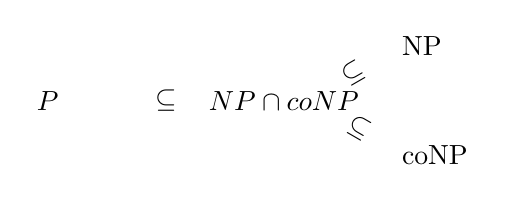
\begin{tikzpicture}
    \node (P) at (1,0) {$P$};
    \node (NPcoNP) at (4,0) {$NP \cap coNP$};
    \node (NP) [above right=0.20cm and 0.3cm of NPcoNP] {NP};
    \node (coNP) [below right=0.20cm and 0.3cm of NPcoNP] {coNP};
    \node at ($(P)!0.5!(NPcoNP)$) {$\subseteq$};
    \node[rotate=30] at ($(NPcoNP)!0.5!(NP)$) {$\subseteq$};
    \node[rotate=-30] at ($(NPcoNP)!0.5!(coNP)$) {$\subseteq$};
\end{tikzpicture}

It si not known if any of the above includes are strict. We dont know if SAT $\in$ coNP and UNSAT $\in$ NP.

The problem of determining the winner of a parity game is in NP $\cap$ coNP, but not known to be in P.

\subsection{Space complexity}

Measure how much working space a TM needs to use (not including space taken by the input).

Assume TMs have a separate input tape with a read-only head and K working tapes with read-write heads.

$\text{SPACE}_M(n) = \max\{ \text{total number of spaces vidited by working tape heads on run } r | \\ 
w \in \Sigma^*, |w| = n, e \text{ is a run of M on input } w\}$

$L \in DSpace(T(n))$: deterministic TM M that decides for language such that 
\begin{equation*}
    space_M (n) = O(T(n))
\end{equation*}

$L \in NSpace(T(n))$: nondeterministic TM M that decides for language such that
\begin{equation*}
    space_M (n) = O(T(n))
\end{equation*}

\begin{equation*}
    PSPACE = \bigcup_{\substack{\Pp: \N \to \N \\ \text{(polynomial)}}} DSpace(p(n))
\end{equation*}

\begin{equation*}
    NPSPACE = \bigcup_{\substack{\Pp: \N \to \N \\ \text{(polynomial)}}} NSpace(p(n))
\end{equation*}

Logaritmic space:
\begin{equation*}
    L = DSPACE(Log(n))
\end{equation*}

Nondeterministic logaritmic space:
\begin{equation*}
    NP = NSPACE(Log(n))
\end{equation*}


Proposition: NP $\subseteq$ PSPACE

\begin{proof}
    Suppose $L \in NP$. By the certificate characterisation of NP there exists a deterministic PTime TM M
    and a polynomial $p(n): \N \to \N$, s.t. $w \in L \iff \exists v \Sigma^{p(n)}$ M accepts w.v.

    We adapt M to a deterministic polyspace TM for L.

    Adapted machine:
    If $w \in \Sigma^n$ is on input tape repeat for every $v \in \Sigma^{p(n)}$ on working tape we write w.v run M on input on working tape, accept 
    w if M accepts w.v. If no certificate is found, at end reject.

    Takes exponential time but only polynomial space.
\end{proof}

\begin{equation*}
    EXP = \bigcup_{\substack{\Pp: \N \to \N \\ \text{(polynomial)}}} DTime(2^{p(n)})
\end{equation*}

\begin{equation*}
    NEXP = \bigcup_{\substack{\Pp: \N \to \N \\ \text{(polynomial)}}} NTime(2^{p(n)})
\end{equation*}


\begin{theorem}
    NPSPACE $\subseteq$ EXP
\end{theorem}

\begin{proof}
    idea: Look at all possible configurations of a nondeterministic TM that uses only polynomial space.
    There are only exponentially many such configurations. Using exponential time we can search the graph of configurations to see
    if there is a path to an accepting state.
\end{proof}

We now have:
\begin{equation*}
    L \subseteq NL \subseteq P \subseteq NP \subseteq PSPACE \subseteq EXP \subseteq NEXP
\end{equation*}

The only inclusions known to be struct are:
\begin{equation*}
    L \subset PSPACE \text{ and } P \subset EXP
\end{equation*}

The only known to be not strict is:
\begin{equation*}
    PSPACE = NPSPACE
\end{equation*}

EXP $\subseteq$ NEXP is not known to be strict. In fact:

\begin{theorem}
    $EXP \neq NEXP => P \neq NP$
\end{theorem}

\begin{proof}
    Suppose $L \in NEXP \setminus EXP$. Let $p(n)$ be a polynomial such that $L$ is decided by nondet TM M that runs in $2^{p(n)}$ steps.
    Consider the language ($L' = \{0^{2^{p(|w|)}}, w | w \in L\}$). We claim $L' \in NP \setminus P$.
    
    $L' \in NP$
    
    Take an input v. Deterministically check if it of the form $0^{2^{p(|w)}}, w$ (othervise reject). Then run the nondet.
    M on input w. This is a polytime nondeterministic machine.
    
    $L' \notin P$
    Suppose there is a deterministic TM M' that decides L' in polynomial time $q(n): \N \to \N$.
    
    We use this to decide L by Given input wl write $0^{2^{p(|w|)}}, w$ onto the tape. Run M' on the above input.
    
    This takes time: $\mathscr{O}(2^{p(|w|)})$ for setting np. $\mathscr{O}(q(c\cdot2^{p(|w|)}))$ for running M'
    $= \mathscr{O}(2^{poly(|w|)})$
\end{proof}





\newpage
% 13.11.2023
\section{PSPACE Completeness}
Todays content:
\begin{itemize}
    \item The TQBF problem
    \item TQBF $\in$ PSPACE
    \item[*] TQBF is NSPACE complete
    \item hence PSPACE = NPSPACE  
\end{itemize}

\subsection{QBF}[quantified boolean formulas]

A quantified boolean formula is:
\begin{itemize}
    \item a boolean variable: $u, b, \dots$
    \item a boolean constant: 0 (false), 1 (true)
    \item if $\Phi, \Psi$ are quantified boolean formulas, then so are: $\Phi \lor \Psi, \Phi \land \Psi, \neg \Phi$
\end{itemize}

Every propositional formula is a qbf (with no quantifiers).

If $\Phi$ is a propositional formula with variables $u_1, \dots, u_k$, then 
\begin{itemize}
    \item $\exists u_1 \dots \exists u_k \Phi$ is true $\iff$ $\Phi$ is satisfiable.
    \item $\forall u_1 \dots \forall u_k \Phi$ is true $\iff$ $\Phi$ is a tautology (valid).
\end{itemize}

A variable in a qbf is free if it does not accur inside the scope of a quantifier.
bound otherwise.

A qbf $\Phi$ is closed if it has no free variables.
A closed qbf has a determined truth value.

\subsection{TQBF problem}
Input: a closed qbf $\Phi$

Question: Is $\Phi$ true?

As a language
\begin{equation*}
    TQBF = \{\Phi | \Phi \text{ is a closed qbf formula and } \Phi \text{ is true}\}
\end{equation*}

Proposition: TQBF $\in$ PSPACE

Proof idea illustrated using one example.

Input: $\forall u \exists v (u \cap v) \cup (\neg u \cap \neg v)$

L is PSPACE hard, if for every PSPACE language $L'$ $L' \leq_p L$.
L is NPSPACE hard, if for every NPSPACE language $L'$ $L' \leq_p L$.

\begin{theorem}[Meyer $\&$ Stockmeyer 1973]
    TQBF is NPSPACE hard. (hence also PSPACE hard).
\end{theorem}
Corollary: PSPACE = NPSPACE
\begin{proof}
    Suppose $L \in $NPSPACE. Let $f$ be a ptime reduction from $L$ to TQBF. Then we have the following deterministic polynomial space algorithm
    for L. Given input $w$
    \begin{enumerate}
        \item compute $f(w)$
        \item decide if $f(w)$ is true.
    \end{enumerate}
\end{proof}

Suppose $L$ is decided by a nondeterministic TM M where space is bounded by $p(n)$ polynomial.

For convenience assume that the machine M loops on the accept, and only ever accepts after erasing all data on the working tapes and reset head positions.

We define the configuration graph of M run on an input word w. Vertices are configurations:
\begin{itemize}
    \item a state $q \in Q$
    \item $w$ on the input tape + input tape head position
    \item $v_1, \dots, v_k \in \Gamma^{p(|w|)}$ representing the relevant data on the K working tape + K head positions. 
\end{itemize}

Such a configuration $c$ can be encoded by word ``c'' $\in \{0, 1\}^{a p(|w|)}$

The edges in the graph $c \to c'$ if M can make one step of computation from configuration $c$ to configuration $c'$.

We construct a propositional formula $\Phi_{M, w}(u_1, \dots, u_N, v_1, \dots, v_N)$, where $N = a \cdot p(|w|)$ such that
\begin{itemize}
    \item The size of $\Phi_{M, w}$ is $\mathscr{O}(n)$.
    \item For \overrightarrow{a}, \overrightarrow{b} $\in \{0, 1\}^N$ \dots
    
    $\Phi_{M, w}(\overrightarrow{a}, \overrightarrow{b}) = 1 \iff \overrightarrow{a} = \ulcorner c \urcorner$ and $\overrightarrow{b} = \ulcorner c' \urcorner$ for 2 node $c, c'$ in the configuration graph and $c \to c'$.
\end{itemize}

The formula $\Phi_{M, w}$ is defined in an analogous why to the formula constructed in the proof of Cook-Levin theorem.

We construct qbformulas $\Psi_i (u_1, \dots, u_N, v_1, \dots, v_N)$. Satisfying
\begin{itemize}
    \item The size of $\Psi_i$ is polynomial in N.
    \item For $c, c'$ in the config graph $\Psi(\ulcorner c \urcorner, \ulcorner c'\urcorner) = 1 \iff $ there is a directed path of length $2^i$ from $c$ to $c'$.
\end{itemize}

Given this we are done, because the required ptime reduction from $L$ to TQBF is:
\begin{itemize}
    \item given the input word $w$, construct $\Psi_{M, w} (\vec{u}, \vec{v})$ as above, and hence $\Psi_N(\vec{u}, \vec{v})$
    \item Then $\Psi_N (\ulcorner start \urcorner, \ulcorner accept \urcorner) = 1$ \\
    $\iff$ $\exists$ path of length $2^N$ from start to accept configuration \\
    $\iff$ $\exists$ path from start to accept configuration \\
    $\iff$ $w \in L$
    \item The closed formula $\Psi_N (\ulcorner start \urcorner, \ulcorner accept \urcorner)$ has size polynomial in $N = cp(|w|)$ hence polynomial in $|w|$
\end{itemize}

% Preveri, ce smo naredili se kaj






\newpage
% 20.11.2023
\section{Logarithmic space}
Recall:
\begin{itemize}
    \item L = DSPACE(log(n))
    \item NL = NSPACE(log(n))
\end{itemize}

Two examples in L
\begin{gather*}
    DIV3 = \{w \in \{0, 1\}^* | \exists n \in \N \; w = bin(n) \text{ and } 3|n\} \\
    MULT = \{bin(m), bin(n), bin(l) | m, n, l \in \N \text{ and } m \cdot n = l\}
\end{gather*}

\subsection{The PATH problem}
Input: A directed graph $G$ and two vertices $s, t \in G$.
Question: Is there a directed path from $s$ to $t$?

As a language
\begin{gather*}
    PATH = \{(G', s', t') | \text{G is a graph given as a adjacent matrix } G', s' \\
    \text{ the binary representation of vertex s, t' the binary representation of vertex t}\}
\end{gather*}

For a graph G with k vertices such a truple has size $\mathscr{O}(k^2)$.

Vertices are represented by words of size $\mathscr{O}(log k)$. This is also $\mathscr{O}(log n)$ when $n = \mathscr{O}(k^2)$.

Proposition: PATH $\in$ NL.

\begin{proof}
    Observation: If there is a path from $s$ to $t$ in $G$ with $k$ vertices, then there is a path of length $ \leq k$.

    Algorithm (nondeterministic):
    \begin{itemize}
        \item Use two working tapes (A and B).
        \item Start of algorithm given input G', s', t' 
        \item Write s' on tape A and bin(1) on tape B.
    \end{itemize}

    *: At every successible step check tape A to see if t' is on tape A => if so accept.

    Check tape B to see if $bin(k)$ (no. of vertices in G) is on B => if so accept.

    Otherwise consider the vertex v with $bin(v)$ on tape (A).

    Nondeterministically choose a vertex $v'$ s.t. $v \to v'$ in G. Write $w''$ on tape A. increment counter on tape B. Go back to *

    We have PATH $\in$ NL.

    We will show PATH is NL-hard. Hence, PATH is NL-complete.
\end{proof}

L is NL-hard if for every NL language L', we have a deterministic logarithmic space reduction from L' to L.

Reduction uses a TM with read only input tape and write only output tape and k working tapes. We only count the space on working tapes.

Notation:
\begin{equation*}
    L' \leq_L L
\end{equation*}

\begin{theorem}
    PATH is NL-complete.
\end{theorem}

\begin{proof}
    Suppose L is decided by a nondeterministic k tape TM M, whose space is bounded by $c \cdot log(n)$.

    (Assume that M erases its working tapes and resets head position of the input tape before entering the accept state).

    As last week consider the configuration graph of M on an input word w. Configurations have:
    \begin{itemize}
        \item a state $q \in q$
        \item $w$ on input tape + head position on input tape
        \item $v_1, \dots, v_k \in \Gamma^{c \cdot log |w|}$ configurations of working tapes + $k$ head positions.
    \end{itemize}

    The space we need to represent an invividual configuration is $\mathscr{O}(log |w|)$. Any configuration $c$ can be represented
    by $c' \in \{0, 1\}^{a \cdot log|w|}$ for some a.

    The required logspace reduction $w \to G, s, t$ where:
    \begin{itemize}
        \item $G$ is the adjacent matrix of the configuration graph of $M$ on $W$
        \item $s$ is the start configuration
        \item $t$ is the accept configuration
    \end{itemize}

    This reduction is only logarithmic space by the following algorithm:
    Construct the adjacency matrix of G by a nested for loop.

    \begin{algorithm}[H]
        \begin{algorithmic}[1]
            \For{$i \in \{0, 1\}^{a \cdot \log |w|}$}
                \For{$j \in \{0, 1\}^{a \cdot \log |w|}$}
                    \If{$i = c'$ and $j = c'$ and $c \rightarrow c'$}
                        \State add 1 to the accept tape
                    \Else
                        \State put 0 otherwise
                    \EndIf
                \EndFor
            \EndFor
        \end{algorithmic}
        \end{algorithm}
\end{proof}








\newpage
% 27.11.2023
\section{Probabilistic TMs and class BPP}

A simple probabilistic TM 
\begin{gather*}
    (start, \_) \to (start, \_, 0)  \\
    (start, \_) \to (accept, \_, 0)
\end{gather*}

The probabilistic TM chooses the transition by tossing a fair coin.

\begin{itemize}
    \item The worst case run time is $\infty$
    \item The probability of termination is 1
    \item The expected run time is $\frac{1}{2} \cdot 1 + \frac{1}{4} \cdot 2 + \frac{1}{8} \cdot 3 \dots = \sum_{n = 1}^{\infty} \frac{n}{2^n} = 2$
\end{itemize}

A probabilistic TM is specified by $(Q, \Gamma, \Delta)$, exactly the same data as a nondeterministic TM. The difference is in the execution model
(how we run the machine).
\begin{itemize}
    \item Start in the start state
    \item Whenever the machine is in a configuration $(q, t, h)$ and there are $K$ possible transitions to $K$ potential successor configurations, the machine chooses
    one of these successors with uniform probability $\frac{1}{k}$.
\end{itemize}

When the machine is executed on an input word $w$ we either get
\begin{itemize}
    \item a finite run $c_1 \to \dots \to c_N$ where $c_N$ is a terminal configuration (always with a positive probability)
    \item an infinite run $c_1 \to c_2 \to \dots$ that never reaches a terminal configuration (might happen with positive probability, or might happen with probability $0$)
\end{itemize}

If M is a PTM:

Worst-case time: ($\equiv$ time for M as a NTM)
\begin{equation*}
    wtime_M(n) = \max \{\text{no. steps in the run r | r is a run of M on input w,} |w| = n\}
\end{equation*}
This is not appropriate for probabilistic computation.

More relevant is Expected time:
\begin{equation*}
    xtime_M(N) = max \{E[\text{number of steps in a run } r \text{ of } M \text{ on } w]| |w| = n\}
\end{equation*}

\begin{example}
    Finding the k-th smallest element in an unsorted array.

    Input: n numbers, k

    Output: find the k-th smallest $a_i$, ie the $k-th$ element if we sort $a_1, \dots, a_n$

    An easy algorithm: sort the array, then select the k-th element from the array. Time complexity is $\mathscr{O}(n)$.

    A probabilistic algorithm with expected time $O(n)$:

    A recursive probabilistic algorithm Find (k; $a_1, \dots, a_n$)
    \begin{itemize}
        \item Randomly choose $i \in \{1, \dots, n\}$
        \item Go through $a_1, \dots, a_n$ in turn and we return a permutation of $a_1, \dots, a_n$ of the form 
        $b_1, \dots, b_l, c_{l+1}, \dots, c_m, d_{m+1}, \dots, d_n$ where $0 \leq l < m \leq n$
        \item if $l + 1 \leq k \leq m$ return $a_i$
        \item if $k \leq k$ recursively compute Find ($k$; $b_1, \dots, b_l$)
        \item if $k > n$ recursively compute Find ($k-m; d_{m+1}, \dots, d_n$) 
    \end{itemize}

    Proposition: $wtime_{Find}(n) = \mathscr{O}(n^2)$

    Proposition: $xtime_{Find}(n) = \mathscr{O}(n)$

    \begin{proof}
        We assume for convenience that all $a_1, \dots, a_n$ are distinct.
        So always $m = l + 1$ = the order rank of $a_i$ in $a_1, \dots, a_n$.
        From the algorithm we have for some constant $c$
        $T(n) \leq c \cdot n + \frac{1}{n}[\sum_{m = 1}^{k-1} + \sum_{m = k + 1}^{n} T(m-1)]$
        $T(1) \leq c$

        We prove by induction the $T(n) \leq 4 c n$
        \begin{align*}
            T(n) \leq& cn + \frac{1}{n} [\sum_{m=1}^{k-1} T(n-m) + \sum_{m = k + 1}^{n} T(m-1)] \\
                 \leq& cn + \frac{4c}{n} [\sum_{m=1}^{k-1} (n-m) + \sum_{m = k + 1}^{n} (m-1)] \\
                 \leq& cn + \frac{4c}{n} \cdot \frac{3}{4} n^2 \\
                 =& 4cn 
        \end{align*}
    \end{proof}

    (visual proof v profesorjevih zapiskih)

\end{example}




\section{Primality testing}
The Miller-Rabin property for prime numbers.

If $p = 2^s \cdot d + 1$ is prime, where $d$ is odd, then for every number $a \in \{1, \dots, p-1$\} one of the following holds;
\begin{itemize}
    \item[a] $a^d \equiv 1 mod n$
    \item[b] $a^{2^r \cdot d} \equiv -1 mod n$ for some $r \in \{0, \dots, s-1\}$
\end{itemize}

If $n = 2^s \cdot d + 1$ is composite ($d$ odd, $s \geq 1$), then at most $\frac{n}{4}$ of $a \in \{1, \dots, n'1\}$ satisfy one of (a) or (b) holds.

Miller-Rabin algorithm for large odd n = $2^s \cdot d + 1$ in
\begin{itemize}
    \item Randomly choose $a \in \{1, \dots, n-1\}$
    \item check if one of (a) or (b) holds
\end{itemize}

if so return \textbf{PROBABLY Prime} if not return \textbf{COMPOSITE}.

If repeated $k$ times the algorithm returns always \textbf{PROBABLY Prime}, then there is only a probability of $\frac{1}{4^k}$ of error.


\section{BPP}

(Bounded Probabilistic Polynomial)

A PTM runs in expected polynomial time if there is a polynomial $p(n)$ such that $xtime_M(n) = \mathscr{O}(p(n))$.

A PTM decides L with bounded error
\begin{itemize}
    \item if on any input $w \in \Sigma^*$, M halts with probability 1 in either accept or reject.
    \item if $w \in L$, P(M on $w$ halts in accept) $\geq \frac{2}{3}$
    \item if $w \notin L$, then P(M on $w$ halts in reject) $\geq \frac{2}{3}$
\end{itemize}

BPP = $\{L | $ there exists an expected ptime probabilistic TM that decides L with bounded error$\}$







\newpage

% 4.12.2023
\section{The graph isomorphism problem (GI)}

Input: $G_1, G_2$, two graphs with the same number of vertices given as adjecency matrices.

Question: Are $G_1$ and $G_2$ isomorphic?

As a language:
\begin{equation*}
    GI = \{\ulcorner G_1 \urcorner, \ulcorner G_2 \urcorner | G_1 \text{ and } G_2 \text{ are isomorphic } (G_1 \cong G_2)\}
\end{equation*}

\begin{equation*}
    GNI = \{\ulcorner G_1 \urcorner, \ulcorner G_2 \urcorner | G_1 \text{ and } G_2 \text{ are not isomorphic } (G_1 \not \cong G_2)\}
\end{equation*}

GI and GNI are not known to be in P.

Babai: GI is quasipolynomial, in fact decidable in $DTime(2^{(\log n)^3})$.

GI is clearly in NP (take the isomorphism itself as the certificate).

GNI is clearly in coNP but not known to be in NP.

How can we ``certify'' that two graphs are not isomorphic?

By considering interactive protocols it is possible for a prover that knows that 2 graphs are not isomorphic to convince a verifier
(that is polynomially time bounded but can use probability) of this fact with a probability of error that can be made arbitrarily small.

This is an example of an interactive proof.

\subsection*{An interactive proof showing that $G_1 \not \cong G_2$}
Assuming the 2 graphs are not isomorphic.

\begin{enumerate}
    \item \textbf{V} picks a random $i \in \{1, 2\}$ by tossing a fair coin and a random permutation $\sigma$ on $\{1, 2, \dots, n\}$ with the uniform distribution.
        
    \textbf{V} communicates $G_3 = \sigma (G_i)$ to the prover.

    \item \textbf{P} chooses $j$ where $j = 1$ if $G_3 = G_1$ else $2$ and communicates $j$ to \textbf{V}.
    
    \item \textbf{V} \textbf{accept} if $j = i$ else \textbf{reject}.
\end{enumerate}

In total:
\begin{itemize}
    \item If the two graphs are not isomorphic then \textbf{V} \textbf{accept}s with probability $1$.
    \item If the two graphs are isomorphic irrespective of the algorithm that \textbf{P} uses for its part of the interaction.
    \item $P(\textbf{accept}) = \frac{1}{2}$
\end{itemize}

\subsection*{Completeness}
There exists a behaviour of P such that if $G_1 \not \cong G_2$ then $P(\textbf{accept}) = 1$.

\subsection*{Soundness}
For any P that conforms to the protocol (returns $j \in \{1, 2\}$)
If $G_1 \cong G_2$ then $P(\textbf{reject}) = \frac{1}{2}$

\subsection*{Argument}
The input to P is a graph uniformly at random from the collection of graphs isomorphic to $G_1$ and $G_2$.
This gives no information about $i$.

The chance of $j$ is independent of $i$. So $Pr(i \neq j) = \frac{1}{2}$.

\subsection{Interactive protocols between \textbf{V} and \textbf{P}}
\textbf{V} is given by a probabilistic TM.

\textbf{P} is any function $\Sigma^* \to \Sigma^*$.

A K-round interaction on input word $w \in \Sigma^*$ is (k can depend on $w$):

\begin{itemize}
    \item \textbf{V} computes $r_1, v_1 = V(w)$
    
    \textbf{P} computes $p_1 = P(w, v)$

    \item \dots
    
    \item \textbf{V} computes $r_k, v_k = V(w, r_1, v_1, p_1, \dots, r_{k-1}, v_{k-1}, p_{k-1})$
    
    \textbf{P} computes $p_k = P(w, v_1, p_1, \dots, v_{k-1}, p_{k-1}, v_k)$

    \item \textbf{V} halts in state $V(w, r_1, v_1, p_1, \dots, r_k, v_k, p_k) \in \{\textbf{accept}, \textbf{reject}\}$
\end{itemize}

\begin{definition}
    IP (languages with interactive proofs)

    $L \in IP $ if there exists an expected polytime probabilistic TM V such that:
    \begin{itemize}
        \item completeness:
        
        $\exists$ proover that interacts with V such that
        \begin{equation*}
            \forall w \in L: Pr(Out<v,p,w>=\textbf{accept}) \geq \frac{2}{3}
        \end{equation*}
        \item soundness:
        
        $\forall$ proovers P that interact with V and
        \begin{equation*}
            \forall w \notin L: Pr(out<v,p,w>=\textbf{reject}) \geq \frac{2}{3}
        \end{equation*}
    \end{itemize}

\end{definition}

Where \textbf{P} interacts with \textbf{V} means
\begin{itemize}
    \item $\forall w, v_1, p_1, v_2, \dots, v_i \; | P(w, v1, p1 \dots) | \: \leq p(|w|)$
    \item $\forall w \in \Sigma^* $ with probability 1 the \textbf{P}, \textbf{V} interaction on $w$ halts in \textbf{accept} or \textbf{reject} in a number of rounds 
    polynomial in the length of $w$.
\end{itemize}







\newpage
% 11.12.2023
\section{Zero-knowledge proofs}

Recall
\begin{equation*}
    GI = \{\ulcorner G_1 \urcorner, \ulcorner G_2 \urcorner | G_1 \cong G_2\}
\end{equation*}

Suppose \textbf{P} knows an isomorphism $\pi: G_1 \to G_2$. \textbf{P} can convince \textbf{V} that the graphs are isomorphic by 
communicating $\pi$ to \textbf{V}.

We will show, that \textbf{P} can convince \textbf{V} that $G_1$ and $G_2$ are isomorphic without giving any information about the isomorphism
$\pi$ (or indeed any other isomorphism).

\subsection{ZKP for GI}
Assume that \textbf{P} knows an isomorphism $\pi: [1, \dots, n] \to [1, \dots, n]$, $\pi (G_1) = G_2$.

\begin{enumerate}
    \item \textbf{P} generates a random permutation $\pi': [1, \dots, n] \to [1, \dots, n]$
    
    \textbf{P} communicates the graph $G_3 = \pi'(G_2)$ to \textbf{V}.

    \item \textbf{V} tosses a coin $i \in \{1, 2\}$ with half-half probability and communicates $i$ to \textbf{P}.
    
    \item \textbf{P} returns to \textbf{V} $\pi'' = $($\pi'$ if $i = 2$ or $\pi' \circ \pi$ if $i = 1$).

    \item \textbf{V} checks that $\pi''(G_i) = G_3$ and if so \textbf{accept}s else \textbf{reject}s.
\end{enumerate}

\begin{itemize}
    \item Completeness:
    
    If $\pi$ is a graph isomorphism with $G_2 = \pi(G_1)$ then \textbf{V} accepts with probability 1.
    
    \item Soundness:
    
    If $G_1 \neq~ G_2$ then for any proover \textbf{P} interacting with \textbf{V} probability of reject $\geq \frac{1}{2}$.
    
    \item Zero-knowledge:
    
    If $G_1 \cong G_2$ amd \textbf{P} behaves following the rules then no $\textbf{V}^*$ learns anything about $\pi$ from the interaction.
\end{itemize}

For any polytime probabilistic $\textbf{V}^*$ that interacts with \textbf{P}, there exists a ptime probabilistic $\textbf{S}^*$ that simulates the result
of $\textbf{V}^*$, \textbf{P} discourse without any recourse to $\pi$. I.e.,
\begin{equation*}
    \forall (\ulcorner G_1 \urcorner, \ulcorner G_2 \urcorner) \in GI \dots
\end{equation*}

$\textbf{S}^*$ we have $G_1 \cong G_2$
\begin{enumerate}
    \item Chooses a random $j \in \{1, 2\}$ (via fair coin) and random permutation $\pi'$ and generates $G_3 = \pi'(G_1)$
    \item $\textbf{S}^*$ uses $\textbf{V}^*$ to do what it does to return $i \in \{1, 2\}$
    \item if $i \neq j$ go back to step 1
    \item simulate the second round of $\textbf{V}^*$ on input $\pi''$
\end{enumerate}

\subsection*{Suppose P knows a 3-colouring C of a graph G}

\begin{enumerate}
    \item \textbf{P} generates a random permutation $\sigma: \{R, G, B\} \to \{R, G, B\}$.
    \item \textbf{V} chooses random edge of a graph.
    \item \textbf{P} opens those envelopes (connected vertices to this edge).
    \item \textbf{V} accepts if the two colours in the envelopes are different, reject if same.
\end{enumerate}

\begin{itemize}
    \item Completeness:
    
    If G is 3-colourable and C is a 3-colouring then $P(\textbf{accept}) = 1$

    \item Soundness:
    
    If there is no 3-colouring then for any $\textbf{P}^*$ we have $P(\textbf{reject}) \geq \frac{1}{n^2}$

    \item Zero-knowledge:
    
    If C is a 3-colouring of G and \textbf{P} is behaving as its supposed to then no probabilistic ptime verifier learns anything about C from the interaction.
\end{itemize}

The sealed envelopes are implemented using bit commitment.

A one-way function is a ptime computable $f: \Sigma^* \to \Sigma^*$ such that for any ptime A there is a negligible function
$\Sigma$ such that for all $n$:
\begin{equation*}
    Pr_{x \in \Sigma^n} [A(f(x)) = x' s \cdot t f(x') = f(x)] < \Sigma(n)
\end{equation*}

Proposition: If 1-way function exists then $P \neq NP$

A one-way permutation is a one-way function with two additional properties:
\begin{itemize}
    \item $f$ is one-to-one (injective)
    \item $\forall w \in \Sigma^* |f(w)| = |w|$
\end{itemize}

Follows that $f$ is a permutation on $\Sigma^n$ % preveri to

Assumption for next part of lecture: a 1-way permutation exists.

\begin{theorem}[Goldreich-Levin theorem]
    Suppose $f$ is a 1-way permutation. Then for every probabilistic ptime algorithm there is a negligible function 
    $\Sigma$ s.t.
    \begin{equation*}
        Pr_{x \in \{0, 1\}^n, r \in \{0, 1\}^n} [A(f(x), r) = x \odot r] \leq \frac{1}{2} + \Sigma(n)
    \end{equation*}
    where
    \begin{equation*}
        [x \odot r = \sum_{i=1}^{n} x_i r_i mod 2]
    \end{equation*}
    To commit a bit b:
    \begin{itemize}
        \item Pick a sufficiently safe n
        \item Randomly choose x, r $\in \Sigma^n$ such that xor = b
        \item Then (f(x), r) is my 'sealed envelope' and can be publicly revealed
        \item To reveal the information, reveal x
    \end{itemize}
\end{theorem}







% Samo za 10-ko
\newpage
% 18.12.2023
\section{$IP = PSPACE$}
\subsection{$IP \subseteq PSPACE$}
An IP for language $L$ is given by a ptime probabilistic \textbf{V} such that:
\begin{itemize}
    \item completeness: There exists some \textbf{P} interacting with \textbf{V} such for any $w \in L$ the interaction accepts with probability $\geq \frac{2}{3}$
    \item soundness: For any $w \notin L$, and any $\textbf{P}^*$ interacting with \textbf{V}, the interaction accepts with probability $\leq \frac{1}{3}$  
\end{itemize}

\textbf{P} not assumed to satisfy any resource bounds, need not be computable.

However there exists an optimum \textbf{P} and this \textbf{P} is in PSPACE.

\begin{theorem}
    $IP \subseteq PSPACE$
\end{theorem}

We can assume \textbf{V} is worst case ptime!

\begin{proof}
    (outline):
    Suppose V is a (worst-case) ptime probabilistic verifier of an IP for L.

    Given a word $w \in \Sigma^*$.
    
    Construct a tree of all possible interactions between all possible $\textbf{P}^*$s and \textbf{V} on input $w$.

    \begin{center}
        \begin{forest}
            [\textbf{V}%: input %$w \in \Sigma^{p(|w|)}$
                [\textbf{P}
                    [\textbf{V}
                        [\textbf{P}
                            [\textbf{V}
                                [...]
                                [...]
                            ]
                            [...]
                        ]
                        [\textbf{accept}]
                    ]
                    [\textbf{V}
                        [...]
                        [\textbf{P}
                            [...]
                            [\textbf{V}
                                [\textbf{reject}]
                                [\textbf{accept}]
                            ]
                        ]
                    ]
                ]
                [\textbf{P}
                    [\textbf{V}
                        [...]
                        [\textbf{reject}]
                    ]
                    [\textbf{V}
                        [...]
                        [...]
                    ]
                ]
            ]
        \end{forest}
    \end{center}

    In first root \textbf{V} recieves $w$ as an input, where $w \in \Sigma^{p(|w|)}$. Then,
    \begin{itemize}
        \item At V nodes calculate weighted average
        \item At P nodes calculate maximum
    \end{itemize}

    The tree takes up more than polynomial space. But using polynomial space we can do a depth first search. At each node we calculate
    the highest probability that \textbf{V} can accept from that node if $\textbf{P}^*$ is as cooperative as possible from that point onward.

    This gives a value to the root of the tree. Accept if root value $\geq \frac{2}{3}$, reject if the root value $\leq \frac{1}{3}$.
\end{proof}

The optimum proover goes down the branch with the highest value.

\subsection*{Warm up for main theorem: $UNSAT \in IP$}
$\#3-SAT_D = \{("\phi", k) | \phi$ is a 3-CNF and $k$ = number of satisfying assignments for $\phi\}$

\begin{theorem}
    $\#3-SAT_D \in IP$
\end{theorem}

\begin{corollary}
    $UNSAT \in IP$
\end{corollary}

We convert a 3-CNF formula $\Phi (x_1, \dots, x_n)$

% (formula) Ne vem ce je potrebno ...

to a polynomial $f_{\Phi} (x_1, \dots, x_n)$

The number of satisfying assignments of $\Phi$ is

\begin{equation*}
    \sum_{b_1 \in \{0, 1\}} \sum_{b_2 \in \{0, 1\}} \dots \sum_{b_n \in \{0, 1\}} f_{\Phi} (b_1, b_2, \dots, b_n)
\end{equation*}

We cant efficiently compute the sum, because it is a sum over $2^n$ vectors.

\textbf{P} sends \textbf{V} a prime $p$ in the range $(2^{|\Phi|}, 2^{|\Phi|+1})$.

\textbf{V} verifies that $p$ is prime (e.g. by AKS algorithm). If not \textbf{reject}.

If $p$ is prime \textbf{V} asks \textbf{P} to convince it that (formula).

Interlude: Checking the value of polynomials over $FF_p$ ([p]).

An $\epsilon$-error value checker for a polynomial $g(x_1, \dots, x_n)$ of degree $\leq d$ is IP that takes $n$ values $a_1, \dots, a_n, c \in [p]$
as input and satisfies:
\begin{itemize}
    \item completeness: if $g(x_1, \dots, x_n) = c$ then the interaction accepts with probability $1$
    \item soundness: if $g(x_1, \dots, x_n) \neq c$ then for any $\textbf{P}^*$ the interaction accepts with prob $\leq \epsilon$.
\end{itemize}

\begin{lemma}
    If $G(x_1, \dots, x_n)$ of degree d has a k-round (of P) $\epsilon$-error value checker then
    $g'(x_1, \dots, x_{n-1}) = \sum_{x_n \in \{0, 1\}} g(x_1, \dots, x_n)$ has a (k+1)-round
    $(\epsilon + \frac{d}{p})$-value checker.
\end{lemma}

\begin{proof}
    We have the following protocol for $a_1, \dots, a_{n-1}, c$. To verify $g'$ = c: $\sum_{x_n \in \{0, 1\}} g(a_1, \dots, a_{n-1}, x_n) = c$:
    \begin{itemize}
        \item \textbf{P} sends V the at most d + 1 coefficients for the univarate polynomial $h(x_n) = g(a_1, \dots, a_{n-1}, x_n)$
        \item \textbf{V} checks if $h(0) + h(1) = c$. If not \textbf{reject}
        \item \textbf{V}chooses random $a_n \in [p]$, sends this to \textbf{P}
        \item $(\textbf{PV})^*$ Follow the assumed IP to check if $h(a_n) = g(a_1, \dots, a_{n-1}, a_n)$
    \end{itemize}
    
    Complete the protocol using the $n$-rounds of \textbf{P} IP provided by $n$ iterations of the lemma above starting with deterministic ptime verifier that
    $f_{\Phi} (a_1, \dots, a_n) = c$ (which is a 0-round 0-error value checker)
\end{proof}


\subsection{Theorem: $TQBF \in IP$}
\begin{theorem}
    $TQBF \in IP$
\end{theorem}
A major result. See notes: christmas reading. See textbook.
\subsection*{Corollary $PSPACE \subseteq IP$}
If $L \in IP$ and $L' \leq_p L$ it is easy to show that $L' \in IP$.

As a consequence $TQBF \in IP \implies PSPACE \subseteq IP$







\newpage
% 8.1.2024
% nadaljevanje od zadnjic
Goal of first hour: Complete proof that $IP = PSPACE$.

Last lecture:
\begin{itemize}
    \item $IP \subseteq PSPACE$
    \item To show $PSPACE \subseteq IP$ it suffies to show $TQBF \in IP$
    \item We showed as a warm-up: $3-SAT \in IP$
\end{itemize}

\subsection{$TQBF \in IP$}
We need an IP to convince us of the truth of a formula
\begin{equation*}
    Q_1 x_1 \dots Q_n x_n \Psi (x_1, \dots, x_n)
\end{equation*}
where $\Psi$ is in 3-CNF.

First idea (as for $3-SAT$) we ``arithmetise'' instead of 
\begin{equation*}
    \forall x_1 \exists x_2 \forall x_3 \exists x_4 \Psi (x_1, x_2, x_3, x_4)
\end{equation*}
(is true iff)

Consider
\begin{equation*}
    \prod_{x_1 \in \{0, 1\}} \sum_{x_2 \in \{0, 1\}} \prod_{x_3 \in \{0, 1\}} \sum_{x_4 \in \{0, 1\}} f_\Psi (x_1, x_2, x_3, x_4)
\end{equation*}
$ \neq 0$

e.g. if $\Psi$ is $(x_1 \lor \neg x_2 \lor x_3) \land (\neg x_1 \lor x_2)$ then
\begin{equation*}
    f_\Psi (1 - ((1 - x_1) \cdot x_2 \cdot (1 - x_3))) \cdot (1 - x_1 (1 - x_2))
\end{equation*}

Issues with using $\sum, \prod$ expansion
\begin{itemize}
    \item Result value is bounded by $2^{2^n}$ rather than $2^n$
    \item the intermediate steps of the protocol involve multiplying polynomials and the degree is not polynomialy bounded.
\end{itemize}

To address the first problem we replace 
\begin{equation*}
    \sum_{b \in \{0, 1\}} a_b
\end{equation*}
with
\begin{equation*}
   \coprod_{b \in \{0, 1\}} a_b = a_0 + a_1 - a_0 a_1 %(prod mora biti obrnjen na glavo)
\end{equation*}
This coincides with disjunction on values $a_b \in \{0, 1\}$.

We change formula from up to this:
\begin{equation*}
    \prod_{x_1 \in \{0, 1\}} \coprod_{x_2 \in \{0, 1\}} \prod_{x_3 \in \{0, 1\}} \coprod_{x_4 \in \{0, 1\}} f_\Psi (x_1, x_2, x_3, x_4)
\end{equation*}

To address the second problem, use the observation for $x \in \{0, 1\}$
\begin{equation*}
    x = x^2 = x^3 = x^4 = \dots
\end{equation*}
Given a polynomial $f(x_1, \dots, x_n)$

Consider
\begin{align*}
    L_i(f) =& x_i \cdot f(x_1, \dots, x_{i-1}, 1, x_{i+1}, \dots, x_n) \\
           +& (1 - x_i) \cdot f(x_1, \dots, x_{i-1}, 0, x_{i+1}, \dots, x_n)
\end{align*}

$L_i(f)$ agrees with $f$ on $x_i \in \{0, 1\}$ and is linear in $x_i$, $deg(L_i(f)) \leq deg(f) + 1$.
The degree of all variables other than $x:i$ is unchanged

Instead, we consider:
\begin{equation*}
    \prod_{x_1} L_1 \coprod_{x_2} L_1 L_2 \prod_{x_3} L_1 L_2 L_3 \coprod_{x_4} L_1 L_2 L_3 L_4 f_\Psi(x_1, x_2, x_3, x_4) = 1
\end{equation*}
degree is always bounded by $max(3m + n - 1, 2n)$. We get $\mathscr{O}(n^2)$

IP protocol for $Q_1 x_1 \dots Q_n x_n \Psi = 1$

\textbf{P} sends \textbf{V} a large enough prime p (to keep error small)

\textbf{V} verifies that $p$ is prime (else \textbf{reject}) and
asks \textbf{P} to convince it that
\begin{equation*}
    \prod_{x_1} L_1 \prod_{x_2} L_1 L_2 \dots \prod_{x_n} L_1 \dots L_n f_\Psi (x_1, \dots, x_n) = 1 %\prod je hkrati prod in amalg  
\end{equation*}
This is done using $\frac{n (n + 3)}{2}$ rounds of interaction using protocols for each operator.

\begin{lemma}
    If we have a polynomial $g(x_1, \dots, x_n)$ of degree $\leq d$ has a k-rounds $\epsilon$-error value checker.
    Then 
    \begin{equation*}
        g_{L_i} (x_1, \dots, x_n) = L_i(g)
    \end{equation*}
    has a (k+1)-rounds $(\epsilon + \frac{d}{p})$-error value checker.
\end{lemma}


\newpage
% Od tu naprej za vse
\section{Complexity classes}
Decision problems are represented by functions $\Sigma^* \to \{0, 1\}$. We have lots of complexity classes for such functions.
Today some complexity classes for more general functions $\Sigma_1^* \to \Sigma_2^*$.

\subsection{FP (Function polytime)}
A function $f: \Sigma_1^* \to \Sigma_2^*$ is in FP if there exsists a multitape TM M that 
computes $f$ and a polynomial $p(n)$ such that
\begin{equation*}
    \forall w \in \Sigma_1^* time_M(w) \leq p(|w|)
\end{equation*}

\begin{remark}
    If $f \in FP$ then there exsists a polynomial $p(n)$ such that $\forall w \in \Sigma_1^*$ $|f(w)| \leq p(|w|)$.
\end{remark}

(We already used this in polytime reducibility.)

\begin{remark}
    \begin{gather*}
        f: \N \to \N \\
        f: \Sigma^* \to \N \\
        f: \N \to \Sigma^*
    \end{gather*}
    We say $f$ is in FP if function that maps binary representations of n to binary frpresentations of $f(n)$ is in FP.%are in FP if in FP with respect to binary representation of numbers.
\end{remark}

\subsection{Counting problems}
Counting problems provide an interesting class of computationally interesting functions.

\subsection{Some examples}

\begin{itemize}
    \item $\#SAT: \Sigma_{PROP}^* \to \N$
    \begin{equation*}
        \#SAT(\Phi) = \text{number of satisfying assignments for } \Phi
    \end{equation*}
    \item $\#3COL: \Sigma_{Graph}^* \to \N$
    \begin{equation*}
        \#3COL(G) = \text{number of 3-colourings of } G
    \end{equation*}
\end{itemize}


\subsubsection{$\#$P}
``Sharp P''

A function $f: \Sigma^* \to \N$ belongs to $\#$P if there exsists a deterministic polytime M
and polynomial $p$ s.t.
\begin{equation*}
    f(w) = |\{v \in \Sigma^{p(|w|)} | M(w, v) \text{ \textbf{accept}s}\}|
\end{equation*}

Recall: $L \in NP$ iff $\exists$ deterministic polytime TM M and polynomial $p$ s.t.
\begin{equation*}
    w \in L \iff \exists v \in \Sigma^{p(|w|)} . M(u, v) \text{ \textbf{accept}s}
\end{equation*}
(the certificate definition of NP)

\begin{remark}
    Obvious that $\#$SAT $\in$ $\#$P, $\#$3COL $\in$ $\#$P ...
\end{remark}

Fact: FP $\subseteq$ $\#P$

Proposition: if $FP = \#P$ then $P = NP$.

\begin{proof}
    Suppose $\#$SAT $\in$ FP. Then we have a P decision procedure for SAT.

    Input: $\Phi$
    Output: $\#$SAT($\Phi$) $\neq 0$

    It is atleast as hard to count certificates as is it to check if a certificate exsists.
\end{proof}

(In words:)
\begin{proof}
    If $FP = \#P$ then we have a deterministic polytime algorithm for counting the number of satisfying assignments of a propositional formula $\Phi$.
    By accepting if this number $\neq 0$ and rejecting if this number $= 0$ we obtain a deterministic polytime decision procedure for SAT.
\end{proof}

More interesting:
    sometimes it is strictly harder to count certificates then to check if a certificate exsists. (assuming $P \neq NP$)

\subsection{Cycles in directed graphs}

Input is a directed graph G.

The decision problem CYCLE:
\begin{itemize}
    \item does G have a (directed) cycle?
\end{itemize}
This is in $P$ (actually solvable in linear time).


The counting problem $\#$CYCLE:
\begin{itemize}
    \item $\#$CYCLE(G) = the number of simple cycles in G.
\end{itemize}

(a simple directed cycle of length $n$ is a sequence $v_0 \to v_1 \to ... \to v_{n-1} \to v_0$ in which no vertex appears twice)

Proposition:
\begin{enumerate}
    \item $CYCLE \in P$
    \item If $\#CYCLE \in FP$ then $P = NP$
\end{enumerate}


\begin{proof}
    We will proove each part individually.
    \begin{enumerate}
        \item By depth-first search
        \item We prove that if $\#$CYCLE $\in$ FP then HAM $\in$ $P$
        Since HAM is NP-complete, $P = NP$.

        Suppose we have an FP algorithm for $\#$CYCLE. We'll define a P procedure for HAM.

        Let G with $n$ vertices be an input graph. Construct a graph G' by replacing every vertex $w$ in G with the following gadget: (not included, see images on moodle)

        % (slikca)

        Resulting graph has $2n(n \lceil log_2 n \rceil + 1)$ vertices.

        Important fact: There are $m = 2^{n \lceil log_2 n \rceil}$ paths from $u$ to $v$ in G'.

        So for each cycle of length $l$ in G there are $2^{ml}$ corresponding cycles in G'.
        (Relies on cycles being identified up to rotation equivalence.) 

        A Hamiltonian cycle in G is a simple cycle of length n.

        If G has a Hamiltonian cycle then G' has at least $2^{n^2 \lceil log_2 n \rceil}$ simple cycles.

        If G does not have a Ham. cycle, then G has at most $n^{n-1}$ simple cycles.

        So G' has at most $n^{n-1} \cdot 2^{m (n-1)}$ simple cycles.

        \begin{align*}
            n^{n-1} \cdot 2^{m (n-1)} =& n^{n-1} \cdot 2^{n \lceil log_2 n \rceil (n-1)} \\
                                      =& n^{n-1} \bar{n}^{n (n - 1)} \\
                                      \leq& \bar{n}^{(n-1) + n (n-1)} \\
                                      =& \bar{n}^{n^2 - 1} \\
                                      <& \bar{n}^{n^2} \\
                                      =& 2^{n^2 \lceil log_2 n \rceil} 
        \end{align*}

        Decide ``G has a Hamiltonian cycle'' by:
        \begin{equation*}
            \#CYCLE(G') \geq 2^{n^2 \lceil log_2 n \rceil} 
        \end{equation*}
    \end{enumerate}
\end{proof}

Given a function $f: \Sigma^* \to \Sigma^*$

A deterministic TM with an oracle for f is a TM with an additional tape (the oracle tape) and a more general transition (partial) function
\begin{equation*}
    \delta: Q + \Gamma^{k+1} \to Q((\Gamma^{k+1} \times \{-1, 0, 1\}^{k+1}) \cup \{call-f\}) % cup = distort union
\end{equation*}
a transition $(q, a_1, \dots, a_{k+1}) \to (q', call-f)$
change the state to q' and replace the word $w$ on the oracle tape with the word $f(w)$.

A function $g: \Sigma_1^* \to \Sigma_2^*$ is in $FP^f$ if there exists an oracle TM 
that computes g in polynomial time.

\begin{lemma}
    If $f \in FP$ and $g \in FP^f$. Then $g \in FP$.
\end{lemma}

A function $f$ is $\#$P-hard if, for every $g \in \#P, g \in FP^f$.

$f$ is $\#$P-complete if $f \in \#P$ and $f$ is $\#$P-hard.

\begin{theorem}
    $\#SAT$ is $\#P$-complete.
\end{theorem}
(no proof)








\newpage
% 15. 1. 2024
Its not that much material for today.
\section{Synthesis based on the permanent}

\subsection*{Reminder}
If $A$ is an $(n \times n)$-matrix
\begin{gather*}
    det(A) = \sum_{\sigma \in perm(n)} \prod_{i = 1}^{n} sgn(\sigma) \cdot A_{i, \sigma(i)} \\
    perm(A) = \sum_{\sigma \in perm(n)} \prod_{i = 1}^{n} A_{i, \sigma(i)}
\end{gather*}

det(A) is important in linear algebra, while perm(A) is important in combinatorics.

The permanent of a $\{0, 1\}$-matrix counts the number of perfect matchings in the bipartite graph whose bipartite-adjacency matrix is A.

(Bipartite-adjacency matrix shows vertices of one side as rows and vertices of other as columns.)

A perfect matching is a collection of edges such that each vertex has exactly one edge in the collection.

The determinant and perminant are both downwards self-recuvible, i.e. they can be computed in polynomial time
given an oracle solving smaller instances.

\begin{equation*}
    det(\begin{bmatrix}
        3 & 1 & 4 \\
        1 & 5 & 9 \\
        2 & 6 & 5
    \end{bmatrix})
    =
    3 \cdot det(\begin{bmatrix}
        5 & 9 \\
        6 & 5
    \end{bmatrix}) 
    - 1 \cdot det(\begin{bmatrix}
        1 & 9 \\
        2 & 5
    \end{bmatrix})
    + 4 \cdot det(\begin{bmatrix}
        1 & 5 \\
        2 & 6
    \end{bmatrix})
\end{equation*}

\begin{equation*}
    perm(\begin{bmatrix}
        3 & 1 & 4 \\
        1 & 5 & 9 \\
        2 & 6 & 5
    \end{bmatrix})
    =
    3 \cdot perm(\begin{bmatrix}
        5 & 9 \\
        6 & 5
    \end{bmatrix}) 
    + 1 \cdot perm(\begin{bmatrix}
        1 & 9 \\
        2 & 5
    \end{bmatrix})
    + 4 \cdot perm(\begin{bmatrix}
        1 & 5 \\
        2 & 6
    \end{bmatrix})
\end{equation*}

Downwards self reduciblility doesnt provide a polytime algorithm. But it is useful in giving IP for the permanent.

Determinant is polynomial time reducible using Gaussian elimination.

I.e. $Det \in FP$

In contrast.

\begin{theorem}
    Computing the permanent of a $\{0, 1\}$-matrix is $\#$P-complete.
\end{theorem}

A word about problems:
\begin{itemize}
    \item The decision problem: ``does a perfect matching exist'' is in P.
    \item The counting problem: ``how many perfect matchings are there'' is $\#$P-complete.
    \item The decision problem: ``given $B$ and $N$ does $B$ have $N$ perfect matchings'' is in PSPACE and has a nice IP.
\end{itemize}

If $perm$ is in FP then P = NP.

\begin{theorem}
    (Toda)
    PH (polynomial heirarchy) $\subseteq$ $P^{\#P}$
\end{theorem}

\begin{corollary}
    If $perm \in FP$ then $PH = P$.
\end{corollary}

\begin{theorem}
    (Lipton)
    Random self-reducibility of perm.

    Suppose we have an oracle that computes $perm$ correctly on a $(1 - \frac{1}{3n})$ 
    fraction of all $(n \times n)$ matrices over a finite field $F$ with $|F| > 3n$.
    Then we can compute $perm$ in polytime (using oracle) on all $(n \times n)$-matrices 
    by a probabilistic algorithmthat, for any input matrix, returns the correct result with 
    probability $\geq \frac{2}{3} - \frac{1}{3n}$.
\end{theorem}

The modern version replaces $(1 - \frac{1}{3n})$  with any constant $c > \frac{1}{2}$.

\begin{proof}
    Let $A$ be the input matrix. Choose (uniformly) a random matrix $R \in F^{n \times n}$.
    Define $B(x) = A - x \cdot R$. Then:
    \begin{itemize}
        \item $Perm(B(x))$ is a degree $n$ univariate polynomial
        \item For any $a \neq 0$, $B(a)$ is random, hence the oracle computes $perm(B(a))$ 
        correctly with probability $\geq 1 - \frac{1}{3n}$.

        Choose $n + 1$ distinct values $a_1, \dots, a_{n + 1}$. Use the oracle $(n + 1)$ times on inputs $B(a_1), \dots, B(a_{n+1})$
        to get values $p_1, \dots, p_{n+1}$. So with probability $\geq 1 - \frac{n + 1}{3n} = \frac{2}{3} - \frac{1}{3n}$ all values
        of $p_i = perm(B_(a_i))$.

        Find (using interpolation) the unique degree $n$ polynomial $q(x)$ that enjoys $q(a_i) = p_1, \dots, q(a_{n + 1}) = p_{n + 1}$.
        Return $q(0)$, which $= perm(A)$ in the case that al $p_i = perm(B(a_i))$.
    \end{itemize}
\end{proof}

\begin{center}
    \enquote{\textit{I find my daughter's mathematics really difficult. \\
    I wish they did some proofs.}}\\ 
    \hfill -- prof. dr. Alexander Keith Simpson, \\
    \hfill 15. 1. 2024
\end{center}


If we have an algorithm $M$ for $perm$
\begin{equation*}
    Avgtime(n) = E_{A \in F^{(n \times n)}} (\text{time taken by M on matrix A})
\end{equation*}

If $Avgtime(n)$ is $\mathscr{O}(p(n))$ ($p$ a polynomial) then there exsists a ptime 
algorithm that correctly computes the permanent on a $\frac{2}{3}$ fraction of all inputs. 

Then by (modern version of theorem) $perm \in P$.

Run the algorithm with polynomial $p(n)$ expected time for at most $4 p(n)$ steps. 
And if it still hasn't stopped return 0.

The above algorithm is correct on $> \frac{2}{3}$ fraction of inputs.

\begin{theorem}
    (Jerrum, Sinclair, Vigoda 2004) Approximating the permanent

    There exists a probabilistic algorithm what given an $(n \times n)$-matrix $A \in \N^{n \times n}$ 
    and $\epsilon, \delta$ satisfies 
    \begin{equation*}
        Pr [\frac{|\text{result algorithm } - perm(A)|}{perm(A)} < \epsilon] \geq 1 - \delta
    \end{equation*}

    whose computation time is polynomial in $n$, $log(\delta^{-1})$, $\epsilon^{-1}$.

    Caveats:
    \begin{itemize}
        \item the result is for non-negative matrices
        \item polynomial in $\epsilon^{-1}$ is not really very good ($(log \epsilon^{-1})$ would be better)
        \item the hidden constants and order of the polynomial are large.
    \end{itemize}
\end{theorem}


\newpage
\section{The big picture}
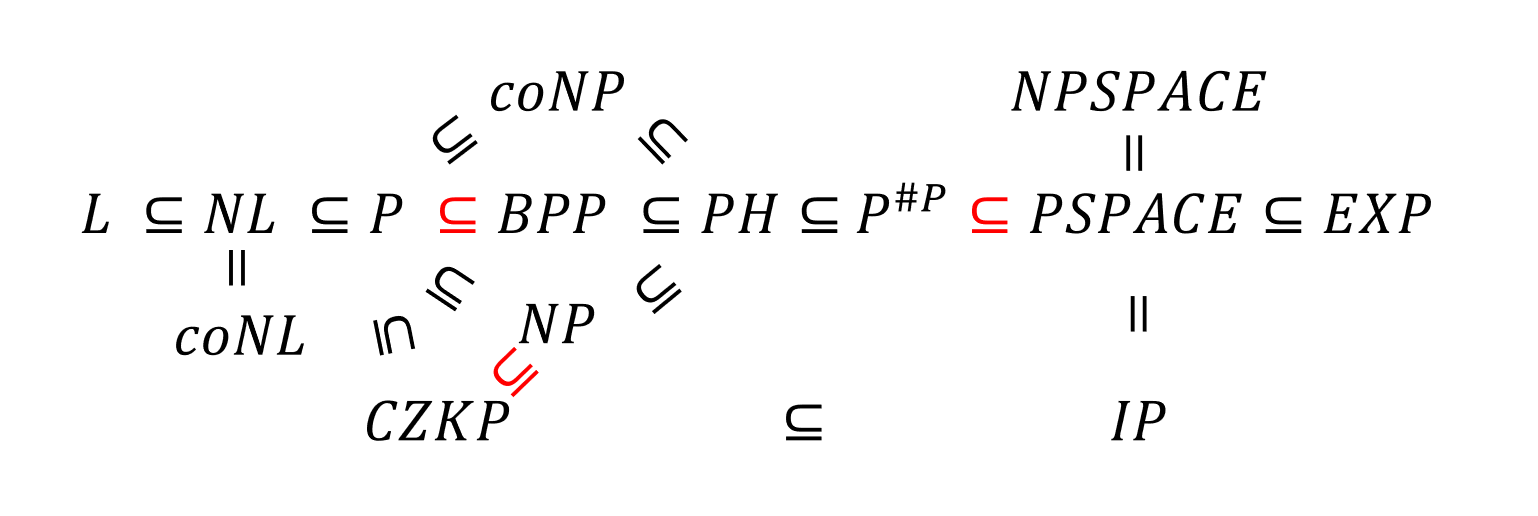
\includegraphics[width=\textwidth]{img/TheBigPicture.png}
Known strict inclusions (hierarchy theorems):
\begin{itemize}
    \item $NL \subset PSPACE$
    \item $P \subset EXP$
\end{itemize}
The red inclusions:
\begin{itemize}
    \item ($\exists$ strong pseude-random generator) $\implies$ $BPP = P$
    \item ($\exists$ one-way function) $\implies$ $CZKP = NP$
    \item The equality $P^{\#P} = PSPACE$ is not known to have any unlikely ???
\end{itemize}
\end{document}